\documentclass[a4paper]{article}

\usepackage[margin=1in]{geometry}
\usepackage{tikz}
\usepackage{pgfplots}
\usepackage{paralist}
\usepackage{amsmath}
\newcommand{\magnitudename}{\text{mag}}
\newcommand{\magnitude}{C_{\magnitudename}}
\newcommand{\varietyname}{\text{var}}
\newcommand{\variety}{C_{\varietyname}}
\newcommand{\lengthname}{\text{len}}
\newcommand{\length}{C_{\lengthname}}
\newcommand{\startactivitiesname}{\text{A-start-\#}}
\newcommand{\startactivities}{C_{\startactivitiesname}}
\newcommand{\startactivitiesrelname}{\text{A-start-rel}}
\newcommand{\startactivitiesrel}{C_{\startactivitiesrelname}}
\newcommand{\startminname}{\text{A-start-min}}
\newcommand{\startmin}{C_{\startminname}}
\newcommand{\startmaxname}{\text{A-start-max}}
\newcommand{\startmax}{C_{\startmaxname}}
\newcommand{\startmeanname}{\text{A-start-mean}}
\newcommand{\startmean}{C_{\startmeanname}}
\newcommand{\startmedianname}{\text{A-start-med}}
\newcommand{\startmedian}{C_{\startmedianname}}
\newcommand{\startdevname}{\text{A-start-dev}}
\newcommand{\startdev}{C_{\startdevname}}
\newcommand{\startvarname}{\text{A-start-var}}
\newcommand{\startvar}{C_{\startvarname}}
\newcommand{\startqonename}{\text{A-start-Q1}}
\newcommand{\startqone}{C_{\startqonename}}
\newcommand{\startqthreename}{\text{A-start-Q3}}
\newcommand{\startqthree}{C_{\startqthreename}}
\newcommand{\startiqrname}{\text{A-start-IQR}}
\newcommand{\startiqr}{C_{\startiqrname}}
\newcommand{\startskewname}{\text{A-start-skew}}
\newcommand{\startskew}{C_{\startskewname}}
\newcommand{\startkurtname}{\text{A-start-kurt}}
\newcommand{\startkurt}{C_{\startkurtname}}
\newcommand{\lastactivitiesname}{\text{A-end-\#}}
\newcommand{\lastactivities}{C_{\lastactivitiesname}}
\newcommand{\lastactivitiesrelname}{\text{A-end-rel}}
\newcommand{\lastactivitiesrel}{C_{\lastactivitiesrelname}}
\newcommand{\lastminname}{\text{A-end-min}}
\newcommand{\lastmin}{C_{\lastminname}}
\newcommand{\lastmaxname}{\text{A-end-max}}
\newcommand{\lastmax}{C_{\lastmaxname}}
\newcommand{\lastmeanname}{\text{A-end-mean}}
\newcommand{\lastmean}{C_{\lastmeanname}}
\newcommand{\lastmedianname}{\text{A-end-med}}
\newcommand{\lastmedian}{C_{\lastmedianname}}
\newcommand{\lastdevname}{\text{A-end-dev}}
\newcommand{\lastdev}{C_{\lastdevname}}
\newcommand{\lastvarname}{\text{A-end-var}}
\newcommand{\lastvar}{C_{\lastvarname}}
\newcommand{\lastqonename}{\text{A-end-Q1}}
\newcommand{\lastqone}{C_{\lastqonename}}
\newcommand{\lastqthreename}{\text{A-end-Q3}}
\newcommand{\lastqthree}{C_{\lastqthreename}}
\newcommand{\lastiqrname}{\text{A-end-IQR}}
\newcommand{\lastiqr}{C_{\lastiqrname}}
\newcommand{\lastskewname}{\text{A-end-skew}}
\newcommand{\lastskew}{C_{\lastskewname}}
\newcommand{\lastkurtname}{\text{A-end-kurt}}
\newcommand{\lastkurt}{C_{\lastkurtname}}
\newcommand{\tlminname}{\text{TL-min}}
\newcommand{\tlmin}{C_{\tlminname}}
\newcommand{\tlavgname}{\text{TL-mean}}
\newcommand{\tlavg}{C_{\tlavgname}}
\newcommand{\tlmaxname}{\text{TL-max}}
\newcommand{\tlmax}{C_{\tlmaxname}}
\newcommand{\tlmedname}{\text{TL-med}}
\newcommand{\tlmed}{C_{\tlmedname}}
\newcommand{\tlmodename}{\text{TL-mode}}
\newcommand{\tlmode}{C_{\tlmodename}}
\newcommand{\tldevname}{\text{TL-dev}}
\newcommand{\tldev}{C_{\tldevname}}
\newcommand{\tlvarname}{\text{TL-var}}
\newcommand{\tlvar}{C_{\tlvarname}}
\newcommand{\tlqonename}{\text{TL-Q1}}
\newcommand{\tlqone}{C_{\tlqonename}}
\newcommand{\tlqthreename}{\text{TL-Q3}}
\newcommand{\tlqthree}{C_{\tlqthreename}}
\newcommand{\tliqrname}{\text{TL-IQR}}
\newcommand{\tliqr}{C_{\tliqrname}}
\newcommand{\tlgmeanname}{\text{TL-g-mean}}
\newcommand{\tlgmean}{C_{\tlgmeanname}}
\newcommand{\tlgdevname}{\text{TL-g-dev}}
\newcommand{\tlgdev}{C_{\tlgdevname}}
\newcommand{\tlhmeanname}{\text{TL-h-mean}}
\newcommand{\tlhmean}{C_{\tlhmeanname}}
\newcommand{\tlskewnessname}{\text{TL-skew}}
\newcommand{\tlskewness}{C_{\tlskewnessname}}
\newcommand{\tlkurtosisname}{\text{TL-kurt}}
\newcommand{\tlkurtosis}{C_{\tlkurtosisname}}
\newcommand{\tlcvariationname}{\text{TL-cvar}}
\newcommand{\tlcvariation}{C_{\tlcvariationname}}
\newcommand{\tlentropyname}{\text{TL-ent}}
\newcommand{\tlentropy}{C_{\tlentropyname}}
\newcommand{\tlhistonename}{\text{TL-hist1}}
\newcommand{\tlhistone}{C_{\tlhistonename}}
\newcommand{\tlhisttwoname}{\text{TL-hist2}}
\newcommand{\tlhisttwo}{C_{\tlhisttwoname}}
\newcommand{\tlhistthreename}{\text{TL-hist3}}
\newcommand{\tlhistthree}{C_{\tlhistthreename}}
\newcommand{\tlhistfourname}{\text{TL-hist4}}
\newcommand{\tlhistfour}{C_{\tlhistfourname}}
\newcommand{\tlhistfivename}{\text{TL-hist5}}
\newcommand{\tlhistfive}{C_{\tlhistfivename}}
\newcommand{\tlhistsixname}{\text{TL-hist6}}
\newcommand{\tlhistsix}{C_{\tlhistsixname}}
\newcommand{\tlhistsevenname}{\text{TL-hist7}}
\newcommand{\tlhistseven}{C_{\tlhistsevenname}}
\newcommand{\tlhisteightname}{\text{TL-hist8}}
\newcommand{\tlhisteight}{C_{\tlhisteightname}}
\newcommand{\tlhistninename}{\text{TL-hist9}}
\newcommand{\tlhistnine}{C_{\tlhistninename}}
\newcommand{\tlhisttenname}{\text{TL-hist10}}
\newcommand{\tlhistten}{C_{\tlhisttenname}}
\newcommand{\tlskewhistname}{\text{TL-hist-skew}}
\newcommand{\tlskewhist}{C_{\tlskewhistname}}
\newcommand{\tlkurthistname}{\text{TL-hist-kurt}}
\newcommand{\tlkurthist}{C_{\tlkurthistname}}
\newcommand{\freqmaxrname}{\text{FREQ-T-max-r}}
\newcommand{\freqmaxr}{C_{\freqmaxrname}}
\newcommand{\freqmaxonename}{\text{FREQ-T-max-1\%}}
\newcommand{\freqmaxone}{C_{\freqmaxonename}}
\newcommand{\freqmaxfivename}{\text{FREQ-T-max-5\%}}
\newcommand{\freqmaxfive}{C_{\freqmaxfivename}}
\newcommand{\freqmaxtenname}{\text{FREQ-T-max-10\%}}
\newcommand{\freqmaxten}{C_{\freqmaxtenname}}
\newcommand{\freqmaxtwentyname}{\text{FREQ-T-max-20\%}}
\newcommand{\freqmaxtwenty}{C_{\freqmaxtwentyname}}
\newcommand{\freqmaxfiftyname}{\text{FREQ-T-max-50\%}}
\newcommand{\freqmaxfifty}{C_{\freqmaxfiftyname}}
\newcommand{\freqmaxseventyfivename}{\text{FREQ-T-max-75\%}}
\newcommand{\freqmaxseventyfive}{C_{\freqmaxseventyfivename}}
\newcommand{\freqmeanname}{\text{FREQ-T-mean}}
\newcommand{\freqmean}{C_{\freqmeanname}}
\newcommand{\freqdevname}{\text{FREQ-T-dev}}
\newcommand{\freqdev}{C_{\freqdevname}}
\newcommand{\freqskewname}{\text{FREQ-T-skew}}
\newcommand{\freqskew}{C_{\freqskewname}}
\newcommand{\freqkurtname}{\text{FREQ-T-kurt}}
\newcommand{\freqkurt}{C_{\freqkurtname}}
\newcommand{\actfreqminname}{\text{FREQ-A-min}}
\newcommand{\actfreqmin}{C_{\actfreqminname}}
\newcommand{\actfreqmaxname}{\text{FREQ-A-max}}
\newcommand{\actfreqmax}{C_{\actfreqmaxname}}
\newcommand{\actfreqmeanname}{\text{FREQ-A-mean}}
\newcommand{\actfreqmean}{C_{\actfreqmeanname}}
\newcommand{\actfreqmedianname}{\text{FREQ-A-med}}
\newcommand{\actfreqmedian}{C_{\actfreqmedianname}}
\newcommand{\actfreqdevname}{\text{FREQ-A-dev}}
\newcommand{\actfreqdev}{C_{\actfreqdevname}}
\newcommand{\actfreqvarname}{\text{FREQ-A-var}}
\newcommand{\actfreqvar}{C_{\actfreqvarname}}
\newcommand{\actfreqqonename}{\text{FREQ-A-Q1}}
\newcommand{\actfreqqone}{C_{\actfreqqonename}}
\newcommand{\actfreqqthreename}{\text{FREQ-A-Q3}}
\newcommand{\actfreqqthree}{C_{\actfreqqthreename}}
\newcommand{\actfreqiqrname}{\text{FREQ-A-IRQ}}
\newcommand{\actfreqiqr}{C_{\actfreqiqrname}}
\newcommand{\actfreqskewname}{\text{FREQ-A-skew}}
\newcommand{\actfreqskew}{C_{\actfreqskewname}}
\newcommand{\actfreqkurtname}{\text{FREQ-A-kurt}}
\newcommand{\actfreqkurt}{C_{\actfreqkurtname}}
\newcommand{\numberuniquetracesname}{\text{DT-\#}}
\newcommand{\numberuniquetraces}{C_{\numberuniquetracesname}}
\newcommand{\percentageuniquetracesname}{\text{DT-\%}}
\newcommand{\percentageuniquetraces}{C_{\percentageuniquetracesname}}
\newcommand{\dtcovname}{\text{DT-cov}}
\newcommand{\dtcov}{C_{\dtcovname}}
\newcommand{\dtrelcovname}{\text{DT-cov-\%}}
\newcommand{\dtrelcov}{C_{\dtrelcovname}}
\newcommand{\dthetname}{\text{DT-het}}
\newcommand{\dthet}{C_{\dthetname}}
\newcommand{\dtsimname}{\text{DT-sim}}
\newcommand{\dtsim}{C_{\dtsimname}}
\newcommand{\daminname}{\text{DA-min}}
\newcommand{\damin}{C_{\daminname}}
\newcommand{\daavgname}{\text{DA-avg}}
\newcommand{\daavg}{C_{\daavgname}}
\newcommand{\damaxname}{\text{DA-max}}
\newcommand{\damax}{C_{\damaxname}}
\newcommand{\dadevname}{\text{DA-dev}}
\newcommand{\dadev}{C_{\dadevname}}
\newcommand{\dadensname}{\text{DA-dens}}
\newcommand{\dadens}{C_{\dadensname}}
\newcommand{\daoverlapname}{\text{DA-ovrlp}}
\newcommand{\daoverlap}{C_{\daoverlapname}}
\newcommand{\complexityfactorname}{\text{comp-fact}}
\newcommand{\complexityfactor}{C_{\complexityfactorname}}
\newcommand{\simpletracedivname}{\text{s-T-div}}
\newcommand{\simpletracediv}{C_{\simpletracedivname}}
\newcommand{\advtracedivname}{\text{a-T-div}}
\newcommand{\advtracediv}{C_{\advtracedivname}}
\newcommand{\loopnumname}{\text{loop-\#}}
\newcommand{\loopnum}{C_{\loopnumname}}
\newcommand{\looprelnumname}{\text{loop-rel-\#}}
\newcommand{\looprelnum}{C_{\looprelnumname}}
\newcommand{\loopavgname}{\text{loop-avg-\#}}
\newcommand{\loopavg}{C_{\loopavgname}}
\newcommand{\loopmaxname}{\text{loop-max-\#}}
\newcommand{\loopmax}{C_{\loopmaxname}}
\newcommand{\loopavgsizename}{\text{loop-avg-size}}
\newcommand{\loopavgsize}{C_{\loopavgsizename}}
\newcommand{\loopmaxsizename}{\text{loop-max-size}}
\newcommand{\loopmaxsize}{C_{\loopmaxsizename}}
\newcommand{\repnumname}{\text{rep-\#}}
\newcommand{\repnum}{C_{\repnumname}}
\newcommand{\reprelnumname}{\text{rep-rel-\#}}
\newcommand{\reprelnum}{C_{\reprelnumname}}
\newcommand{\dfgnodesname}{\text{DFG-V}}
\newcommand{\dfgnodes}{C_{\dfgnodesname}}
\newcommand{\dfgedgesname}{\text{DFG-E}}
\newcommand{\dfgedges}{C_{\dfgedgesname}}
\newcommand{\dfgcncname}{\text{DFG-cnc}}
\newcommand{\dfgcnc}{C_{\dfgcncname}}
\newcommand{\dfgavgdegname}{\text{DFG-adeg}}
\newcommand{\dfgavgdeg}{C_{\dfgavgdegname}}
\newcommand{\dfgmaxdegname}{\text{DFG-mdeg}}
\newcommand{\dfgmaxdeg}{C_{\dfgmaxdegname}}
\newcommand{\dfgdensname}{\text{DFG-dens}}
\newcommand{\dfgdens}{C_{\dfgdensname}}
\newcommand{\dfgstructname}{\text{DFG-struct}}
\newcommand{\dfgstruct}{C_{\dfgstructname}}
\newcommand{\dfgcycnumbername}{\text{DFG-CN}}
\newcommand{\dfgcycnumber}{C_{\dfgcycnumbername}}
\newcommand{\dfgdiamname}{\text{DFG-diam}}
\newcommand{\dfgdiam}{C_{\dfgdiamname}}
\newcommand{\dfgsepnumname}{\text{DFG-sep-\#}}
\newcommand{\dfgsepnum}{C_{\dfgsepnumname}}
\newcommand{\dfgseprationame}{\text{DFG-sep-r}}
\newcommand{\dfgsepratio}{C_{\dfgseprationame}}
\newcommand{\dfgseqrationame}{\text{DFG-seq-r}}
\newcommand{\dfgseqratio}{C_{\dfgseqrationame}}
\newcommand{\dfgcycname}{\text{DFG-cyc}}
\newcommand{\dfgcyc}{C_{\dfgcycname}}
\newcommand{\dfgpathcomplexityname}{\text{DFG-P-comp}}
\newcommand{\dfgpathcomplexity}{C_{\dfgpathcomplexityname}}
\newcommand{\numberofneighborhoodsname}{\text{succ}}
\newcommand{\numberofneighborhoods}{C_{\numberofneighborhoodsname}}
\newcommand{\numberoftiesname}{\text{ties}}
\newcommand{\numberofties}{C_{\numberoftiesname}}
\newcommand{\lempelzivname}{\text{LZ}}
\newcommand{\lempelziv}{C_{\lempelzivname}}
\newcommand{\structurename}{\text{struct}}
\newcommand{\structure}{C_{\structurename}}
\newcommand{\affinityname}{\text{affinity}}
\newcommand{\affinity}{C_{\affinityname}}
\newcommand{\deviationfromrandomname}{\text{dev-R}}
\newcommand{\deviationfromrandom}{C_{\deviationfromrandomname}}
\newcommand{\avgdistname}{\text{avg-dist}}
\newcommand{\avgdist}{C_{\avgdistname}}
\newcommand{\enttracename}{\text{ENT-trace}}
\newcommand{\enttrace}{C_{\enttracename}}
\newcommand{\entprefixname}{\text{ENT-pref}}
\newcommand{\entprefix}{C_{\entprefixname}}
\newcommand{\entprefixflatname}{\text{ENT-pref-F}}
\newcommand{\entprefixflat}{C_{\entprefixflatname}}
\newcommand{\entgblockname}{\text{ENT-g-block}}
\newcommand{\entgblock}{C_{\entgblockname}}
\newcommand{\entgblockflatname}{\text{ENT-g-block-F}}
\newcommand{\entgblockflat}{C_{\entgblockflatname}}
\newcommand{\entlempelzivname}{\text{ENT-LZ}}
\newcommand{\entlempelziv}{C_{\entlempelzivname}}
\newcommand{\entlempelzivflatname}{\text{ENT-LZ-F}}
\newcommand{\entlempelzivflat}{C_{\entlempelzivflatname}}
\newcommand{\entkblockdonename}{\text{ENT-k-block-d1}}
\newcommand{\entkblockdone}{C_{\entkblockdonename}}
\newcommand{\entkblockdthreename}{\text{ENT-k-block-d3}}
\newcommand{\entkblockdthree}{C_{\entkblockdthreename}}
\newcommand{\entkblockdfivename}{\text{ENT-k-block-d5}}
\newcommand{\entkblockdfive}{C_{\entkblockdfivename}}
\newcommand{\entkblockronename}{\text{ENT-k-block-r1}}
\newcommand{\entkblockrone}{C_{\entkblockronename}}
\newcommand{\entkblockrthreename}{\text{ENT-k-block-r3}}
\newcommand{\entkblockrthree}{C_{\entkblockrthreename}}
\newcommand{\entkblockrfivename}{\text{ENT-k-block-r5}}
\newcommand{\entkblockrfive}{C_{\entkblockrfivename}}
\newcommand{\entknnthreename}{\text{ENT-knn-3}}
\newcommand{\entknnthree}{C_{\entknnthreename}}
\newcommand{\entknnfivename}{\text{ENT-knn-5}}
\newcommand{\entknnfive}{C_{\entknnfivename}}
\newcommand{\entknnsevenname}{\text{ENT-knn-7}}
\newcommand{\entknnseven}{C_{\entknnsevenname}}
\newcommand{\epavariantname}{\text{epa-var}}
\newcommand{\epavariant}{C_{\epavariantname}}
\newcommand{\epanormvariantname}{\text{epa-n-var}}
\newcommand{\epanormvariant}{C_{\epanormvariantname}}
\newcommand{\epasequencename}{\text{epa-seq}}
\newcommand{\epasequence}{C_{\epasequencename}}
\newcommand{\epanormsequencename}{\text{epa-n-seq}}
\newcommand{\epanormsequence}{C_{\epanormsequencename}}
\newcommand{\epasequencelname}{\text{epa-seq-L}}
\newcommand{\epasequencel}{C_{\epasequencelname}}
\newcommand{\epanormsequencelname}{\text{epa-n-seq-L}}
\newcommand{\epanormsequencel}{C_{\epanormsequencelname}}
\newcommand{\epasequenceename}{\text{epa-seq-E}}
\newcommand{\epasequencee}{C_{\epasequenceename}}
\newcommand{\epanormsequenceename}{\text{epa-n-seq-E}}
\newcommand{\epanormsequencee}{C_{\epanormsequenceename}}

\begin{document}

\section*{Information About the Performed Analysis}

You chose to analyze the following complexity measures:
\begin{compactenum}
\item $\length$ (n traces)
\item $\numberuniquetraces$ (n variants)
\item $\percentageuniquetraces$ (ratio variants per number of traces)
\item $\magnitude$ (n events)
\item $\tlmin$ (trace len min)
\item $\tlmax$ (trace len max)
\item $\tlavg$ (trace len mean)
\item $\tlmed$ (trace len median)
\item $\tlmode$ (trace len mode)
\item $\tldev$ (trace len std)
\item $\tlvar$ (trace len variance)
\item $\tlqone$ (trace len q1)
\item $\tlqthree$ (trace len q3)
\item $\tliqr$ (trace len iqr)
\item $\tlgmean$ (trace len geometric mean)
\item $\tlgdev$ (trace len geometric std)
\item $\tlhmean$ (trace len harmonic mean)
\item $\tlskewness$ (trace len skewness)
\item $\tlkurtosis$ (trace len kurtosis)
\item $\tlcvariation$ (trace len coefficient variation)
\item $\tlentropy$ (trace len entropy)
\item $\tlhistone$ (trace len hist1)
\item $\tlhisttwo$ (trace len hist2)
\item $\tlhistthree$ (trace len hist3)
\item $\tlhistfour$ (trace len hist4)
\item $\tlhistfive$ (trace len hist5)
\item $\tlhistsix$ (trace len hist6)
\item $\tlhistseven$ (trace len hist7)
\item $\tlhisteight$ (trace len hist8)
\item $\tlhistnine$ (trace len hist9)
\item $\tlhistten$ (trace len hist10)
\item $\tlskewhist$ (trace len skewness hist)
\item $\tlkurthist$ (trace len kurtosis hist)
\item $\freqmaxr$ (ratio most common variant)
\item $\freqmaxone$ (ratio top 1 variants)
\item $\freqmaxfive$ (ratio top 5 variants)
\item $\freqmaxten$ (ratio top 10 variants)
\item $\freqmaxtwenty$ (ratio top 20 variants)
\item $\freqmaxfifty$ (ratio top 50 variants)
\item $\freqmaxseventyfive$ (ratio top 75 variants)
\item $\freqmean$ (mean variant occurrence)
\item $\freqdev$ (std variant occurrence)
\item $\freqskew$ (skewness variant occurrence)
\item $\freqkurt$ (kurtosis variant occurrence)
\item $\dtcov$ (coverage variants)
\item $\dtrelcov$ (rel coverage variants)
\item $\dthet$ (heterogeneity rate variants)
\item $\dtsim$ (similarity rate variants)
\item $\variety$ (n unique activities)
\item $\actfreqmin$ (activities min)
\item $\actfreqmax$ (activities max)
\item $\actfreqmean$ (activities mean)
\item $\actfreqmedian$ (activities median)
\item $\actfreqdev$ (activities std)
\item $\actfreqvar$ (activities variance)
\item $\actfreqqone$ (activities q1)
\item $\actfreqqthree$ (activities q3)
\item $\actfreqiqr$ (activities iqr)
\item $\actfreqskew$ (activities skewness)
\item $\actfreqkurt$ (activities kurtosis)
\item $\startactivities$ (n unique start activities)
\item $\startmin$ (start activities min)
\item $\startmax$ (start activities max)
\item $\startmean$ (start activities mean)
\item $\startmedian$ (start activities median)
\item $\startdev$ (start activities std)
\item $\startvar$ (start activities variance)
\item $\startqone$ (start activities q1)
\item $\startqthree$ (start activities q3)
\item $\startiqr$ (start activities iqr)
\item $\startskew$ (start activities skewness)
\item $\startkurt$ (start activities kurtosis)
\item $\startactivitiesrel$ (rel unique start activities)
\item $\lastactivities$ (n unique end activities)
\item $\lastmin$ (end activities min)
\item $\lastmax$ (end activities max)
\item $\lastmean$ (end activities mean)
\item $\lastmedian$ (end activities median)
\item $\lastdev$ (end activities std)
\item $\lastvar$ (end activities variance)
\item $\lastqone$ (end activities q1)
\item $\lastqthree$ (end activities q3)
\item $\lastiqr$ (end activities iqr)
\item $\lastskew$ (end activities skewness)
\item $\lastkurt$ (end activities kurtosis)
\item $\lastactivitiesrel$ (rel unique end activities)
\item $\enttrace$ (eventropy trace)
\item $\entprefix$ (eventropy prefix)
\item $\entprefixflat$ (eventropy prefix flattened)
\item $\entgblock$ (eventropy global block)
\item $\entgblockflat$ (eventropy global block flattened)
\item $\entlempelziv$ (eventropy lempel ziv)
\item $\entlempelzivflat$ (eventropy lempel ziv flattened)
\item $\entkblockdone$ (eventropy k block diff 1)
\item $\entkblockdthree$ (eventropy k block diff 3)
\item $\entkblockdfive$ (eventropy k block diff 5)
\item $\entkblockrone$ (eventropy k block ratio 1)
\item $\entkblockrthree$ (eventropy k block ratio 3)
\item $\entkblockrfive$ (eventropy k block ratio 5)
\item $\entknnthree$ (eventropy knn 3)
\item $\entknnfive$ (eventropy knn 5)
\item $\entknnseven$ (eventropy knn 7)
\item $\epavariant$ (epa variant entropy)
\item $\epanormvariant$ (epa normalized variant entropy)
\item $\epasequence$ (epa sequence entropy)
\item $\epanormsequence$ (epa normalized sequence entropy)
\item $\epasequencel$ (epa sequence entropy linear forgetting)
\item $\epanormsequencel$ (epa normalized sequence entropy linear forgetting)
\item $\epasequencee$ (epa sequence entropy exponential forgetting)
\item $\epanormsequencee$ (epa normalized sequence entropy exponential forgetting)
\item $\simpletracediv$ (simple trace diversity)
\item $\advtracediv$ (advanced trace diversity)
\item $\damin$ (distinct activities min)
\item $\damax$ (distinct activities max)
\item $\daavg$ (distinct activities mean)
\item $\dadev$ (distinct activities std)
\item $\dadens$ (event density)
\item $\daoverlap$ (distinct activities non overlap)
\item $\complexityfactor$ (complexity factor)
\item $\loopnum$ (n traces with loop)
\item $\looprelnum$ (avg traces with loop)
\item $\loopavg$ (avg loops per trace)
\item $\loopmax$ (max loops per trace)
\item $\loopavgsize$ (avg loop size per trace)
\item $\loopmaxsize$ (max loop size per trace)
\item $\repnum$ (n traces with repetition)
\item $\reprelnum$ (avg traces with repetition)
\item $\numberofneighborhoods$ (number of successions)
\item $\numberofties$ (number of ties)
\item $\structure$ (structure)
\item $\affinity$ (average affinity)
\item $\lempelziv$ (lempel ziv complexity)
\item $\deviationfromrandom$ (deviation from random)
\item $\avgdist$ (average edit distance)
\item $\dfgnodes$ (n nodes dfg)
\item $\dfgedges$ (n edges dfg)
\item $\dfgcnc$ (coeff of connectivity dfg)
\item $\dfgavgdeg$ (avg node degree dfg)
\item $\dfgmaxdeg$ (max node degree dfg)
\item $\dfgdens$ (density dfg)
\item $\dfgstruct$ (structure dfg)
\item $\dfgcycnumber$ (cyclomatic number dfg)
\item $\dfgsepnum$ (n cut vertices dfg)
\item $\dfgsepratio$ (separability ratio dfg)
\item $\dfgseqratio$ (sequentiality ratio dfg)
\item $\dfgcyc$ (cyclicity dfg)
\end{compactenum}

\bigskip
\noindent
Out of these measures, the following were excluded because they returned non-numeric values:
\begin{compactenum}
\item $\tlskewness$ (trace len skewness)
\item $\tlkurtosis$ (trace len kurtosis)
\item $\freqskew$ (skewness variant occurrence)
\item $\freqkurt$ (kurtosis variant occurrence)
\item $\startskew$ (start activities skewness)
\item $\startkurt$ (start activities kurtosis)
\item $\lastskew$ (end activities skewness)
\item $\lastkurt$ (end activities kurtosis)
\end{compactenum}

\bigskip
\noindent
Furthermore, the following measures were excluded because their variance is $0$ in the analyzed data:
\begin{compactenum}
\item $\length$ (n traces)
\item $\dtcov$ (coverage variants)
\end{compactenum}

\bigskip
\noindent
Additionally, the following measures were excluded because they are correlated with other measures:
\begin{compactenum}
\item $\percentageuniquetraces$ (ratio variants per number of traces)
\item $\tlavg$ (trace len mean)
\item $\dtrelcov$ (rel coverage variants)
\item $\dfgnodes$ (n nodes dfg)
\item $\entkblockrone$ (eventropy k block ratio 1)
\item $\looprelnum$ (avg traces with loop)
\item $\reprelnum$ (avg traces with repetition)
\item $\dfgavgdeg$ (avg node degree dfg)
\end{compactenum}

\bigskip
\noindent
This leaves us with a total of $128$ log measures to analyze.

\subsection*{Validity of the Factor Analysis}
Your sample size in this analysis was $2112$.
It is recommended to have a sample size of at least $5 \cdot 146 = 730$.

\noindent 
Bartlett's test of sphericity returned a $\chi^2$ value of $1321643.419324327$ and a $p$-value of $0.0$.
This means, the variables are probably correlated and we can perform a factor analysis.

\noindent
The measure of sampling adequacy (MSA) returned the following results:
\begin{compactitem}
\item $\numberuniquetraces$: $0.9521$
\item $\magnitude$: $0.9344$
\item $\tlmin$: $0.9632$
\item $\tlmax$: $0.9721$
\item $\tlmed$: $0.9886$
\item $\tlmode$: $0.9907$
\item $\tldev$: $0.8897$
\item $\tlvar$: $0.9047$
\item $\tlqone$: $0.9715$
\item $\tlqthree$: $0.9674$
\item $\tliqr$: $0.9543$
\item $\tlgmean$: $0.9318$
\item $\tlgdev$: $0.8566$
\item $\tlhmean$: $0.9315$
\item $\tlcvariation$: $0.6882$
\item $\tlentropy$: $0.7195$
\item $\tlhistone$: $0.6888$
\item $\tlhisttwo$: $0.891$
\item $\tlhistthree$: $0.8824$
\item $\tlhistfour$: $0.654$
\item $\tlhistfive$: $0.7404$
\item $\tlhistsix$: $0.6117$
\item $\tlhistseven$: $0.7078$
\item $\tlhisteight$: $0.6925$
\item $\tlhistnine$: $0.856$
\item $\tlhistten$: $0.6409$
\item $\tlskewhist$: $0.8819$
\item $\tlkurthist$: $0.8898$
\item $\freqmaxr$: $0.8324$
\item $\freqmaxone$: $0.975$
\item $\freqmaxfive$: $0.8917$
\item $\freqmaxten$: $0.9036$
\item $\freqmaxtwenty$: $0.8457$
\item $\freqmaxfifty$: $0.8209$
\item $\freqmaxseventyfive$: $0.9571$
\item $\freqmean$: $0.9162$
\item $\freqdev$: $0.9152$
\item $\dthet$: $0.7606$
\item $\dtsim$: $0.7519$
\item $\variety$: $0.704$
\item $\actfreqmin$: $0.8737$
\item $\actfreqmax$: $0.9722$
\item $\actfreqmean$: $0.9341$
\item $\actfreqmedian$: $0.9722$
\item $\actfreqdev$: $0.8861$
\item $\actfreqvar$: $0.9002$
\item $\actfreqqone$: $0.9282$
\item $\actfreqqthree$: $0.9477$
\item $\actfreqiqr$: $0.941$
\item $\actfreqskew$: $0.8473$
\item $\actfreqkurt$: $0.7899$
\item $\startactivities$: $0.8213$
\item $\startmin$: $0.7807$
\item $\startmax$: $0.7112$
\item $\startmean$: $0.8069$
\item $\startmedian$: $0.8244$
\item $\startdev$: $0.7942$
\item $\startvar$: $0.8836$
\item $\startqone$: $0.8877$
\item $\startqthree$: $0.8677$
\item $\startactivitiesrel$: $0.7171$
\item $\lastactivities$: $0.8988$
\item $\lastmin$: $0.8136$
\item $\lastmax$: $0.9151$
\item $\lastmean$: $0.8522$
\item $\lastmedian$: $0.8705$
\item $\lastdev$: $0.7412$
\item $\lastvar$: $0.9164$
\item $\lastqone$: $0.9268$
\item $\lastqthree$: $0.8923$
\item $\lastactivitiesrel$: $0.7307$
\item $\enttrace$: $0.9559$
\item $\entprefix$: $0.9298$
\item $\entprefixflat$: $0.9216$
\item $\entgblock$: $0.9202$
\item $\entgblockflat$: $0.9171$
\item $\entlempelziv$: $0.9351$
\item $\entlempelzivflat$: $0.9014$
\item $\entkblockdone$: $0.6808$
\item $\entkblockdthree$: $0.8091$
\item $\entkblockdfive$: $0.9485$
\item $\entkblockrthree$: $0.8061$
\item $\entkblockrfive$: $0.8338$
\item $\entknnthree$: $0.9213$
\item $\entknnfive$: $0.9153$
\item $\entknnseven$: $0.9151$
\item $\epavariant$: $0.966$
\item $\epanormvariant$: $0.7655$
\item $\epasequence$: $0.95$
\item $\epanormsequence$: $0.7835$
\item $\epasequencel$: $0.9489$
\item $\epanormsequencel$: $0.7367$
\item $\epasequencee$: $0.9486$
\item $\epanormsequencee$: $0.7584$
\item $\simpletracediv$: $0.8646$
\item $\advtracediv$: $0.8852$
\item $\damax$: $0.9465$
\item $\daavg$: $0.9261$
\item $\dadev$: $0.9207$
\item $\dadens$: $0.8069$
\item $\daoverlap$: $0.8892$
\item $\complexityfactor$: $0.9079$
\item $\loopnum$: $0.8283$
\item $\loopavg$: $0.8291$
\item $\loopmax$: $0.9313$
\item $\loopavgsize$: $0.9071$
\item $\loopmaxsize$: $0.8588$
\item $\repnum$: $0.9224$
\item $\numberofneighborhoods$: $0.9443$
\item $\numberofties$: $0.9431$
\item $\lempelziv$: $0.9776$
\item $\deviationfromrandom$: $0.7758$
\item $\dfgedges$: $0.8709$
\item $\dfgcnc$: $0.8683$
\item $\dfgmaxdeg$: $0.9679$
\item $\dfgdens$: $0.7419$
\item $\dfgstruct$: $0.7448$
\item $\dfgcycnumber$: $0.8446$
\item $\dfgsepnum$: $0.94$
\item $\dfgsepratio$: $0.6112$
\item $\dfgcyc$: $0.9349$
\item $\avgdist$: $0.9221$
\item $\damin$: $0.9664$
\item overall MSA: $0.882187383709089$
\end{compactitem}

\bigskip
\noindent
During the analysis, the MSA values of the following complexity measures were too low:
\begin{compactitem}
\item $\startiqr$: $0.2879$
\item $\lastiqr$: $0.324$
\item $\structure$: $0.281$
\item $\affinity$: $0.4221$
\item $\dfgseqratio$: $0.2501$
\end{compactitem}
These complexity measures were left out of the analysis to produce dependable results.

\subsection*{Chosen Number of Factors}
\noindent
The Scree test resulted in the following Eigenvalue plot:
\begin{center}
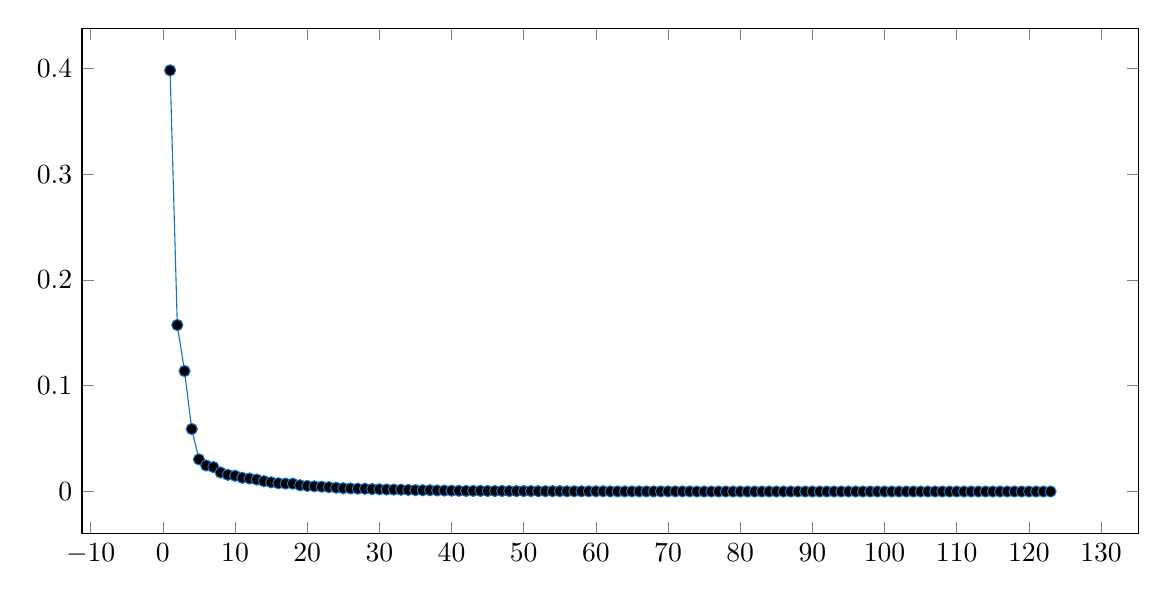
\begin{tikzpicture}
\begin{axis}[width=15cm,height=8cm]
\addplot [draw=cyan!50!blue, mark=*] coordinates { (1,0.3982) (2,0.1574) (3,0.1139) (4,0.0591) (5,0.0304) (6,0.0246) (7,0.0231) (8,0.018) (9,0.0158) (10,0.0149) (11,0.013) (12,0.0123) (13,0.0113) (14,0.0098) (15,0.0087) (16,0.0078) (17,0.0075) (18,0.0074) (19,0.0059) (20,0.0053) (21,0.0049) (22,0.0046) (23,0.0041) (24,0.0036) (25,0.0031) (26,0.0029) (27,0.0027) (28,0.0026) (29,0.0023) (30,0.0021) (31,0.0019) (32,0.0018) (33,0.0017) (34,0.0015) (35,0.0013) (36,0.0012) (37,0.0012) (38,0.001) (39,0.0009) (40,0.0008) (41,0.0007) (42,0.0006) (43,0.0006) (44,0.0006) (45,0.0005) (46,0.0005) (47,0.0005) (48,0.0004) (49,0.0004) (50,0.0004) (51,0.0004) (52,0.0003) (53,0.0003) (54,0.0003) (55,0.0003) (56,0.0002) (57,0.0002) (58,0.0002) (59,0.0002) (60,0.0002) (61,0.0002) (62,0.0001) (63,0.0001) (64,0.0001) (65,0.0001) (66,0.0001) (67,0.0001) (68,0.0001) (69,0.0001) (70,0.0001) (71,0.0001) (72,0.0001) (73,0.0001) (74,0.0) (75,0.0) (76,0.0) (77,0.0) (78,0.0) (79,0.0) (80,0.0) (81,0.0) (82,0.0) (83,0.0) (84,0.0) (85,0.0) (86,0.0) (87,0.0) (88,0.0) (89,0.0) (90,0.0) (91,0.0) (92,0.0) (93,0.0) (94,0.0) (95,0.0) (96,0.0) (97,0.0) (98,0.0) (99,0.0) (100,0.0) (101,0.0) (102,0.0) (103,0.0) (104,0.0) (105,0.0) (106,0.0) (107,0.0) (108,0.0) (109,0.0) (110,0.0) (111,0.0) (112,0.0) (113,0.0) (114,0.0) (115,0.0) (116,0.0) (117,0.0) (118,0.0) (119,0.0) (120,0.0) (121,0.0) (122,0.0) (123,0.0)};
\end{axis}
\end{tikzpicture}
\end{center}
\noindent
You choose to set the number of expected factors to $10$.

\end{document}